\section{Introduction}
This paper has been written to help out novel users of McStas and neutron
scattering instruments. McStas is a software package for simulating
neutron scattering experiments using a Monte Carlo ray-tracing technique. This paper 
aims at helping the user to gain insight into basic neutron scattering 
as well as neutron raytracing using the McStas software package
\cite{McStas0},\cite{Manual},\cite{Websites}.
\subsection{Prerequisites}
Needed knowledge and equipment work through the tutorial is
\begin{itemize}
\item{Undergraduate knowledge of mathematics and physics}
\item{A computer with McStas installed (refer to the McStas
    \htmladdnormallink{homepage}{http://mcstas.risoe.dk}
    \cite{Websites} for details) or a bootable McStas Ubuntu live DVD
    (installation to harddisk possible, but not required)}
\item{This paper}
\end{itemize}
\subsection{Goals and tasks}
The goals and tasks of this paper are
\begin{itemize}
\item{To teach you about the most basic neutron scattering}
\item{To let you understand some of the typical components in a
    neutron scattering instrument}
\item{To teach you basic usage of the McStas neutron simulation
    package}
\item{To let you create your first McStas instruments, a two axis diffractometer and a triple axis spectrometer}
\item{To teach you how to modify your instrument for a specific task}
\item{To help you learn to debug instruments}
\item{To help you aquire and analyze data from McStas simulations}
\end{itemize}
\section{Basic neutron scattering}
You may recall the Bragg law from your high school physics
\[n\lambda=2d\sin(\theta),\]
giving the scattering condition for 
a wave of wavelength $\lambda$ against a series of
lattice planes with lattice spacing $d$, rotated the angle $\theta$
off the lattice plane normal. $n$ is an integer giving the spectral
order of the scattered wave. In neutron science one often refers to
the \emph{scattering vector}, $\vec{\kappa}$ of a given reflection, where
\[\kappa=|\vec{\kappa}|=n\frac{2\pi}{d}.\]
This gives us the scattering vector formulation of the Bragg law
\[\kappa=2k\sin(\theta),\]
where $k=\frac{2\pi}{\lambda}$.
%such that
%\[n\lambda=4\pi \kappa^{-1}\sin(\theta)\]
The Bragg law / scattering condition is illustrated in Figure \ref{bragg.eps}.
\begin{figure}[htb!]
\begin{center}
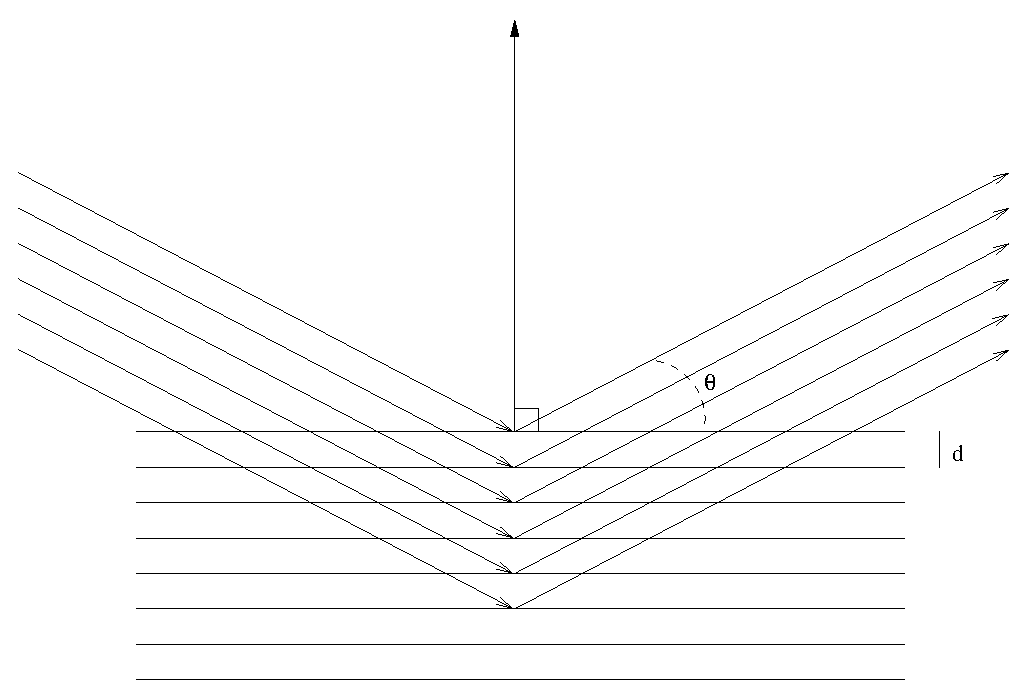
\includegraphics[width=9cm]{pics/bragg.eps}
\end{center}
\caption{Illustration of the Bragg Law.}
\label{bragg.eps}
\end{figure}
Most of the neutron processes we will study in this paper are elastic,
meaning that the wavelength of the neutron is unaltered by the process.
\section{Basic understanding of instrument components}
In the McStas formulation of a neutron scattering instrument, all
objects apart from the neutron ray are referred to as components. This
includes for instance
\begin{itemize}
\item{{\bf Source} The exit of a neutron production facility, where
    neutron rays of certain velocities are emitted into some
    portion of space}
\item{{\bf Monochromator} (Idealized) crystal used to select a
    neutrons of a single wavelength $\lambda_0$ \footnote{In reality,
    the monochromator selects a normal distribution of wavelegths
    around $\lambda_0$, and perhaps higher orders as well ($n=2,3,...$
    in Braggs law)} to probe the sample with (monochromator) or to 
    analyze (analyzer)}
\item{{\bf Sample} An object altering the neutron physical properties
    in some sense, examples used here are}
  \begin{itemize}
    \item{Vanadium. Scatters incoming neutron rays incoherently}
    \item{PowderN. Can be thought of as a large number of crystals,
        each scattering neutron rays according to the Bragg law, thereby
        producing N concentric Debye Scherrer cones. This sample also
        has the posibility of adding inchoherent, eleasticly scattered
        neutron rays.}
    \end{itemize}
\item{{\bf Monitors} Objects \emph{monitoring} or registering neutron ray
    characteristics. In the exercises below are used different types
    of detectors or monitors:}
  \begin{itemize}
    \item{Monitor. Single monitor, detecting the number of flying
        through a plane. (User defined opening size)}
    \item{PSD\_monitor. Square monitor, detecting the number of
        neutron rays passing through a plane, divided into
        pixels. Square regions of a plane. (User defined resolution 
        and opening size)}
    \item{PSD\_monitor\_4PI. As PSD\_monitor but shaped like a sphere.}
    \item{L\_monitor. Wavelength monitor, measuring the different
        wavelengths of the passing neutron rays. (L is for $\lambda$)}
    \item{Monitor\_nD. General monitor for detecting all sorts of
        physical properties of the neutron ray. In our cases used with
        options }
      \begin{itemize}
      \item{'single' - as PSD\_monitor but only one small square}
      \item{'banana' - as PSD\_monitor but shaped like a curved,
          horizontal band }
      \end{itemize}
    \end{itemize}
  \item{{\bf Collimators}} Devices controling the direction and divergence
   of the neutron ray.
    \begin{itemize}
      \item{Collimator\_linear} A series of parallel absorbing neutron plates
       that limits the beam divergence. 
       Typical values are $6'$ to $120'$.
    \end{itemize}
  \end{itemize}
More information on the McStas components is available by using the
\verb+mcdoc+ program (You may need to set the BROWSER system variable
to your webbrowser of choice):
\begin{itemize}
\item{\verb+mcdoc -s+ , Shows a html list of all the components}
\item{\verb+mcdoc Monitor.comp+ , Shows the documentation for a given component}
\item{\verb+mcdoc -M+ , brings up the McStas manual in PDF format}
\item{\verb+mcdoc -c+ , brings up the McStas component manual in PDF format}
\end{itemize}

\section{Basic McStas}
In short, the core of the McStas system is a precompiler. From a
user-provided instrument description, components are assembled into 
a single piece of \texttt{ansi-c} code. Using a compiler, e.g. 
\texttt{gcc}, the c code is compiled into an executable program 
which can be run on your computer. Optionally, the program takes 
input arguments to tune the setup of your instrument/simulation. 
This section will take you through a simple example instrument 
to teach you the basic instrument language of McStas. (Instrument 
filename is vanadium\_example.instr, can be loaded using the
\verb+Neutron Site/Tutorial+ menu item of the \verb+mcgui+, see below)
Please study \emph{carefully} the instructive comments,
marked by \verb+/* ... */+ characters
    
\begin{verbatim}
/* The line below defines the 'name' of our instrument */
/* Here, we have a single input parameter, ROT         */
DEFINE INSTRUMENT vanadium_example(ROT=0)

/* The DECLARE section allows us to declare variables  */
/* in c syntax. Here, coll_div (collimator divergence) */
/* is set to 60 arc minutes...                         */
DECLARE
%{
  double coll_div = 60;
%}

/* Here comes the TRACE section, where the actual      */
/* instrument is defined....                           */
TRACE

/* The Arm() class component defines reference points  */
/* and directions in 3D space. Every component instance*/
/* must have a unique name. Here, arm is used. This    */
/* Arm() component is set to define the origin of our  */
/* global coordinate system (AT (0,0,0) ABSOLUTE)      */
COMPONENT arm = Arm() AT (0,0,0) ABSOLUTE

/* Next, we need some neutrons. Let's place a neutron  */
/* source. Refer to documentation of Source_flat to    */
/* understand the different input parameters.          */
/* The source component is placed RELATIVE to the arm  */
/* component, meaning that modifying the position or   */
/* orientation of the arm will also affect the source  */
/* component (and other components after that one...)  */
COMPONENT source = Source_simple(radius = 0.015, dist = 1,
  xw=0.024, yh=0.015, E0=5, dE=0.2)
 AT (0,0,0) RELATIVE arm

/* Here we have a collimator - placed to improve beam  */
/* divergence. The component is placed at a distance   */
/* RELATIVE to a previous component...                 */
COMPONENT collimator = Collimator_linear(len = 0.2, 
  divergence = coll_div, xwidth = 0.04, yheight=0.06)
  AT (0, 0, 0.4) RELATIVE arm

/* We also need something to 'shoot at' - here a sample*/
/* made from vanadium - an isotrope scatterer. Options */
/* are available to restrict the solid angle in which  */
/* neutrons are emitted (no need to simulate neutrons  */
/* that we know for sure will not reach the rest of    */
/* instrument).                                        */
/* Other options for smart targeting are available -   */
/* refer to component documentation for info.          */
COMPONENT target = V_sample(radius_i = 0.008, radius_o = 0.012, 
  h = 0.015, focus_r = 0, pack = 1,
  target_x = 0, target_y = 0, target_z = 1)
  AT (0,0,1) RELATIVE arm

/* Here, a secondary arm - or reference point, placed  */
/* on the sample position. The ROT parameter above     */
/* defines rotation of this arm (and components        */
/* relative to the arm)                                */
COMPONENT arm2 = Arm() 
  AT (0,0,0) RELATIVE target
  ROTATED (0,ROT,0) relative arm

/* For data output, let us place a detector. This      */
/* detector is not very realistic, since it is sphere  */
/* shaped and has a 10 m radius, but has the advantage */
/* that EVERYTHING emitted from the sample will be     */
/* picked up. Notice that this component changes       */
/* orientation with the ROT input parameter of the     */
/* instrument.                                         */
COMPONENT PSD_4pi = PSD_monitor_4PI(radius=10, nx=101, ny=51,
  filename="vanadium.psd")
  AT (0,0,0) RELATIVE arm2
END
\end{verbatim}
Enlightened by the above example, you are probably now ready to learn
a few more important details and tips about McStas.
\begin{itemize}
\item{{\bf Neutron representation:} A neutron 'history' or package is
  an entity representing a large number of neutrons. It has the
  following physical properties:
  \begin{itemize}
    \item{Spatial coordinates, $\vec{x}$ or $x,y,z$}
    \item{Velocity components, $\vec{v}$ or $v_x,v_y,v_z$}
    \item{Spin components, $\vec{s}$ or $s_x,s_y,s_z$}
    \item{Time, $t$}
    \item{Neutron weight factor, $p$}
  \end{itemize}
\item{{\bf Neutron histories/Intensities:} McStas simulates neutron
    histories rather than direct neutron counts, i.e. when a
    Monte Carlo choice is made in a given component (e.g. a random
    number is generated to decide a new direction of the neutron ray), 
    the neutron \emph{weight factor} is adjusted accordingly. As you
    may have guessed already, the weight factor is the 
    average number of of observed neutrons of a given behaviour.
    The transition to direct neutron intensites is made
    by adjusting the initial neutron weight of the source component,
    so that the sum of all simulated weight factors equals the
    absolute intensity of neutrons emitted in one
    second. This means that the intensity of the neutron beam at a
    given position is the initial neutron weight multiplied by the 
    product of all the Monte Carlo weight factors occuring from the
    source to the given position.  When observing McStas output, $I$
    is the intensity, not $N$.}
\item{{\bf 3D space:} The 3D space in which the instrument is defined,
  usually has a single component which is
  placed ABSOLUTEly  in space, e.g. at (0,0,0). All other components
  can be placed RELATIVE to this component.}
\item{{\bf Changing coordinate system:} Each component has its own
    local coordinate system. As the neutron travels from one component
    to the other, the local component coordinate system changes. The
    definition is that $z$ is the direction toward the next component,
    and that the $y$ direction is vertical. Our coordinate system is 
    right-handed, making $x$ horisontal and pointing left, looking in 
    the direction of $z$.}
\item{{\bf Component order matters!} It is important to understand
    that McStas is component order dependent. The basic idea is to
    follow the neutron as it travels from one component to the next in
    the instument description. This means that if you place one component
    \emph{geometrically} before another component, but \emph{orderly}
    after the other component, neutrons may never reach your 'first'
    component. This means that some designs can be difficult to
    achieve, though generally a solution can be found.}
\item{{\bf Use Arm()'s!} The Arm() component is very good for defining
  changed orientation of the instrument, e.g. for axis turning points
  etc. Placing many Arm()'s will improve future flexibility of your
  instrument.}
\item{{\bf Use PSD\_monitor()'s!} The PSD\_monitor() component is a
    {\bf p}osition {\bf s}ensitive {\bf d}etector. This component can
    be used to image the shape of your beam as it travels through the
    instrument. This is very useful for debugging purposes. Other
    monitors, for instance wavelength monitors can also be useful.}}
\end{itemize}
In the McStas manual, available by clicking
\htmladdnormallink{here}{http://mcstas.risoe.dk/documentation/manual/mcstas-1.8-manual.pdf}
if you are using an internet browser to view this document, description
of usage of the different McStas tools is printed. The main McStas
programs are
\begin{itemize}
\item{\emph{mcstas} - Core application}
\item{\emph{mcgui} - Main graphical user interface}
\item{\emph{mcdisplay} - Ray trace / debugging application}
\item{\emph{mcplot} - Data / display application}
\item{\emph{mcdoc} - Documentation application}
\end{itemize}
Here are a few hints on using the tools:
\begin{itemize}
\item To start mcgui, execute \verb+mcgui+ in a terminal window
  (\verb+mcgui.pl+ on Windows)
\item To handle instrument files (opening, editing, compiling), use \verb+File+ menu of \verb+mcgui+
\item To simulate and plot data, use the \verb+Simulation+ menu of \verb+mcgui+
\item To use the distributed example McStas instruments, use the \verb+Neutron Site+ menu of \verb+mcgui+
\item For further help on usage, use the items of the \verb+mcgui+
  menu of \verb+Help+ menu or read the chapter \emph{Running McStas}
  of the McStas manual \cite{Manual}.
\end{itemize}
\section{Exercises}
Throughout the rest of this paper, you will have to do the work!
Through a series of small exercises, you will set up and use two simple
neutron scattering instruments: a two axis diffractometer and a triple axis spectrometer. To get an idea of what your final
instrument might look like, see the sample instrument protrayed in Figure \ref{instr.eps}.
\begin{figure}[htb!]
\begin{center}
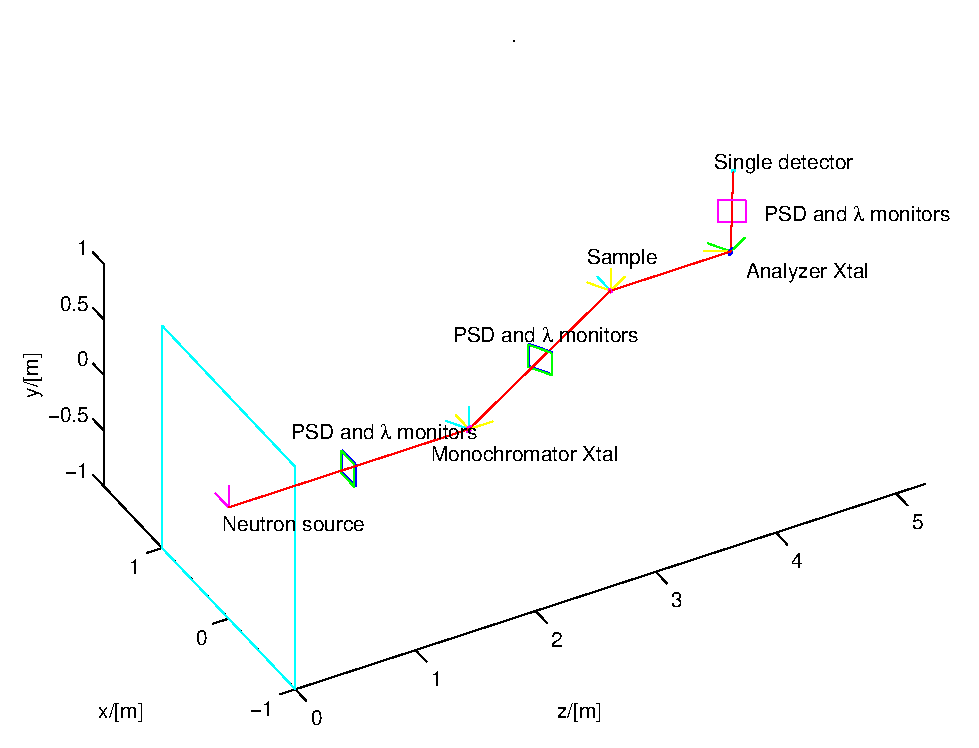
\includegraphics[width=12cm]{pics/instr.eps}
\end{center}
\caption{Illustration of a triple axis diffractometer}
\label{instr.eps}
\end{figure}
\subsection{Exercise: Source and PSD}
\begin{enumerate}
\item{Start by inserting a template instrument (Insert menu). Set up an instrument, consisting only of an Arm (keep the example 'a1' Arm instance), a Source\_Maxwell\_3,
a PSD\_monitor and an L\_monitor. Read the documentation for each of
the components to find the needed input parameters. For the source we
will help you out, try
\begin{verbatim}
COMPONENT source = Source_Maxwell_3(
    size = 0.1, l_low = 0.1, l_high = 10, dist = 10, xw = 0.01,
    yh = 0.01, T1 = 300, T2=300, T3=300, I1=1e14, I2=0, I3=0)
\end{verbatim}
Read the Source\_Maxwell\_3 docs using mcdoc to understand the
suggested parameters. The file names for monitors, specified as character strings, should be given \emph{surrounded} by double quotes ("file.dat").}
\item{Run a simulation and plot the results, looking
at an image of the source plus the wavelength distribution of the
source. }
\item{Narrow down the interval of wavelengths emitted from the
source to e.g. l\_low=0.999 and l\_high=1.001. Rerun your simulation to
check the effect. Reset the wavelength interval to [0.1 10] \AA.}
\item{Estimate the solid angle covered by your PSD. Try if you can
  understand I, the neutron intensity in the PSD, in the two previous
  runs. Try running the simulation with half or double the number of
  neutron rays. Try also to vary the source focus area. Explain what you observe.}
\end{enumerate}
\subsection{Exercise: Insert a monochromator}
\begin{enumerate}
\item{Keeping your current components, insert a Monochromator\_flat
component (use mcdoc or the component manual to get the needed parameters) and a
new set of PSD and L\_monitor after the monochromator. You should now add
two new input parameters of your instrument, e.g. OMM (Omega
Monochromator) and TTM (Two Theta Monochromator)
for rotation of the monochromator and the remaining part of the 
instrument so that the orientation of
monochromator is as portrayed in Figure \ref{mono.eps}.
\begin{figure}[htb!]
\begin{center}
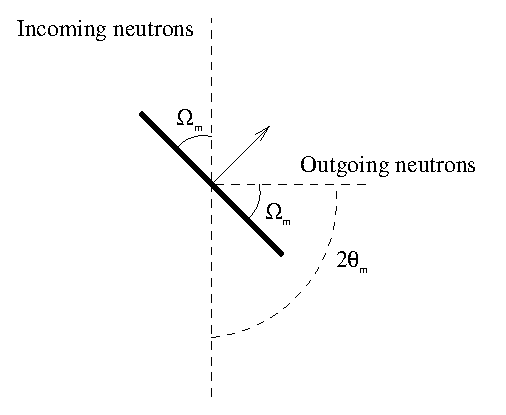
\includegraphics[width=6cm]{pics/mono.eps}
\end{center}
\caption{Illustration of the monochromator orientation}
\label{mono.eps}
\end{figure}
These two instrument input parameters should be added to the DEFINE line of the instrument (start of file). Remember to add an Arm() at the rotation point. }
\item{Given $\lambda$ = 4\AA, and knowing that for the
monochromator $\kappa=1.8734$ \AA$^{-1}$ (Pyrolytic Graphite), use Bragg's law to determine the 
correct Bragg angle (i.e. OMM/TTM) for the monochromator for the $n=1$ reflection. }
\item{Do a scan of OMM a couple of angles around this value to verify
    the finding, keeping TTM fixed. This will be achieved by setting the OMM value to 'min,max' (replace by relevant numerical values) in the Run Simulation window, and selecting the Scan check button in that same window. Enter the number of steps to compute (e.g. 10). Check the position of the peak on
    the PSD and the wavelength on the L\_monitor. }
\item{What should $\kappa$ be set to to get the $n=2$ reflection at exactly
    OMM=45$^\circ$ (TTM=90$^\circ$)?
Adjust $\kappa$ for the monochromator and verify the calculation by a
scan, check the wavelength. }
\item{Determine the Bragg angle for the $n=1$ reflection in this
setting of $\kappa$, and verify by scaning OMM. Set OMM to this
value. Perform the simulation and check the wavelength distribution.
Comment.}
\item{Before you go on, change the minimum and maximum wavelengths of
    the source to a suitably narrow interval around the wavelength you select,
    e.g. 4\AA. (No need to
    produce neutron rays that will not be scattered at the monochromator...)}
\end{enumerate}
\subsection{Exercise: Insert a sample}
\begin{enumerate}
\item{Now, insert a \verb+V_sample()+ component (Vanadium scatters
    incoherently, i.e. in all
    directions) after the last PSD\_monitor and L\_monitor. Insert a Beamstop component after the sample, e.g. AT
    (0,0,0.5) RELATIVE sample. 
    At the
    same position as the sample, insert a PSD\_monitor\_4PI\_log component of radius
    1.0 m., located AT (0,0,0) RELATIVE to your sample.
    Read the documentation for details on input parameters.
    Run a simulation. Notice the number of hits.}
\end{enumerate}
\subsection{Exercise: Insert a different sample}
\begin{enumerate}
\item{Next, let us insert something more interesting. Remove the
    V\_sample and  PSD\_monitor\_4PI\_log. Insert a PowderN component
    with the following parameters:
    \begin{verbatim}
COMPONENT sample = PowderN(radius=0.01,h=0.01, d_phi0=0.1, pack=0.5, 
   DW=0.9, frac=0.5, focus_r=0.03, reflections="mylist.dat",
   Vc=3.86*3.86*11.82, sigma_a=0, sigma_inc=2, barns=1)
  AT (0, 0, 0) RELATIVE a4
\end{verbatim}
You should also create a list of reflections, e.g. \texttt{mylist.dat}
with the following contents:
\begin{verbatim}
# column_j 3 multiplicity 'j'
# column_q 1  Scattering vector modulus [Angs^-1]
# column_F2 2 Scattering factor |F^2| in [barns]
1 1000 8
1.3 1000 4
\end{verbatim}

(Adjust placement relative to your component naming etc.). Also insert
  a banana shaped detector,
\begin{verbatim}
COMPONENT ND = Monitor_nD(xwidth=1, options="banana, theta limits=[-45 45],auto y")
  AT (0,0,0) RELATIVE a5
\end{verbatim}
and take away the previously inserted Beamstop. Test that neutrons
reach the detector, then run a long simulation (many neutron rays) and have coffee.}
\end{enumerate}
\subsection{Exercise: Insert an analyzer}
\begin{enumerate}
\item{Insert a single detector by changing the options for the
    Monitor\_nD component to ``single''. Also, add an angle to rotate
    the part of the instrument located after the sample, e.g. TT (Two
    $\Theta$) and decide a more relevant size of the now rectangular detector. Look at your results from the last simulation to
    determine an approximate scan range for the TT angle. Also,
    set a small focus\_r on the sample component to minimize
    calculation time on non-detected neutron rays. Scan TT across the
    powder lines.}
\item{Between sample and detector, set up an analyser crystal by
    copying and modifying your monochromator component. (Add new arms
    and angles OMA, TTA - A is for Analyzer - for adjusment.) 
    Adjust the analyser to Bragg condition
    for the chosen wavelength. Re-scan TT and notice the difference to
    the scan performed in the previous task. Try also scanning around
    -TT and notice the difference to the other scan. Can you explain
    the difference?}
\end{enumerate}
\section{Suffix}
Well done, you have come to the end of the McStas tutorial. Hopefully,
most of the goals of the tutorials have been fulfilled. Otherwise,
feel free to contact the
\htmladdnormallink{authors}{mailto:peter.willendrup@risoe.dk,kim.lefmann@risoe.dk}
of this paper or the \htmladdnormallink{McStas users
  mailinglist}{mailto:neutron-mc@risoe.dk} for further help.

\begin{thebibliography}{10}
\bibitem{McStas0}
K. Lefmann and K. Nielsen: \emph{McStas, a general software package
  for neutron ray-tracing simulations}, Neutron News, {\bf 10} pp. 20-23, 1999

\bibitem{Manual}
P. Willendrup, E. Farhi K. Lefmann et. al.: \emph{User and Programmers
  Guide to the Neutron Ray-Tracing Package McStas, Version 1.11},Ris\o\
National Laboratory, Roskilde, Denmark, January 2007\\
\bibitem{Component Manual}
P. Willendrup, E. Farhi K. Lefmann et. al.: \emph{Component Manual for
 the Neutron Ray-Tracing Package McStas, Version 1.11},Ris\o\
National Laboratory, Roskilde, Denmark, January 2007\\

\bibitem{Websites}
McStas homepages:\\
\newblock Official website at Ris\o, \url{http://www.mcstas.org}\\
\newblock Supplementary ILL website, \url{http://www.ill.fr/tas/mcstas}\\
\end{thebibliography}


